\documentclass[11pt]{article}

% ==== Paquetes ====
\usepackage[utf8]{inputenc}
\usepackage[T1]{fontenc}
\usepackage[spanish]{babel}
\usepackage{amsmath, amssymb, amsfonts}
\usepackage{graphicx}
\usepackage{caption}
\usepackage{subcaption}
\usepackage{float}
\usepackage{geometry}
\usepackage{hyperref}
\usepackage{minted}
\usepackage{mdframed}
\geometry{margin=2.3cm}

\usemintedstyle{friendly}
\setminted{fontsize=\scriptsize, breaklines=true}

% ==== Datos de la tarea ====
\title{IEE3584 – Comunicaciones Inalámbricas \\ \large Tarea 14}
\author{Nicolás Seguel}
\date{}

\begin{document}
\maketitle

\section*{Pregunta 32: Decodificación ZF}

En esta pregunta se realizan simulaciones Monte Carlo para estimar el BER promedio utilizando decodificación \textbf{Zero-Forcing (ZF)} en configuraciones MIMO con modulación QPSK sobre un canal Rayleigh plano.

% ===========================================
\subsection*{32.a) Simulación ZF para configuraciones 1x1, 2x1, 4x1 y 8x1}

En este inciso se simulan sistemas MISO con un receptor y distintos números de antenas transmisoras.  
Las figuras siguientes muestran el BER simulado para cada configuración junto a las curvas teóricas 1x1.

\begin{figure}[H]
    \centering
    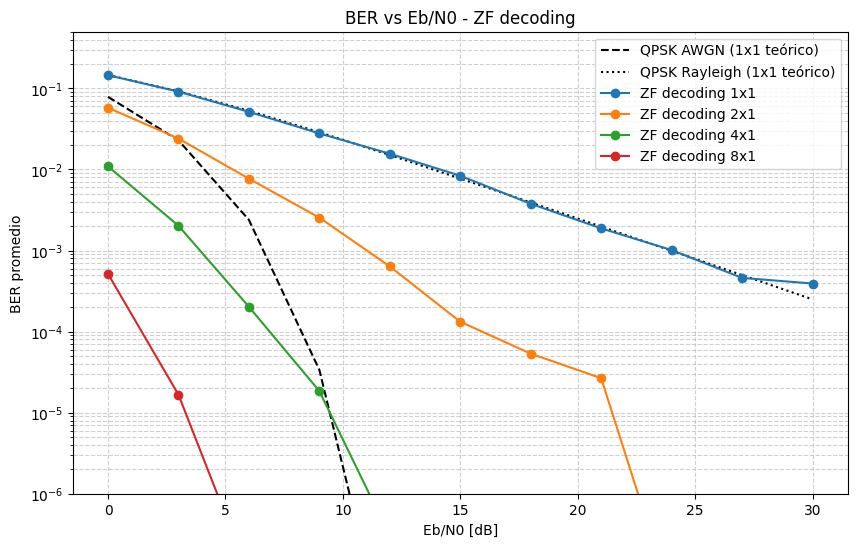
\includegraphics[width=0.95\textwidth]{fig_zf_1x1_2x1_4x1_8x1.png}
    \caption{BER vs $E_b/N_0$ para configuraciones ZF: 1×1, 2×1, 4×1 y 8×1.}
\end{figure}

A mayor número de antenas transmisoras, se aprecia una mejora significativa en la pendiente de decaimiento del BER, especialmente en 4×1 y 8×1. Esto es esperable debido a la ganancia de diversidad en el enlace ascendente. La curva 1×1 coincide con el desempeño teórico en AWGN, validando la implementación.


% ===========================================
\subsection*{32.b) Simulación ZF para configuraciones 1x1, 2x2, 4x4 y 8x8}

Ahora se evalúan configuraciones cuadradas MIMO con el mismo número de antenas transmisoras y receptoras.

\begin{figure}[H]
    \centering
    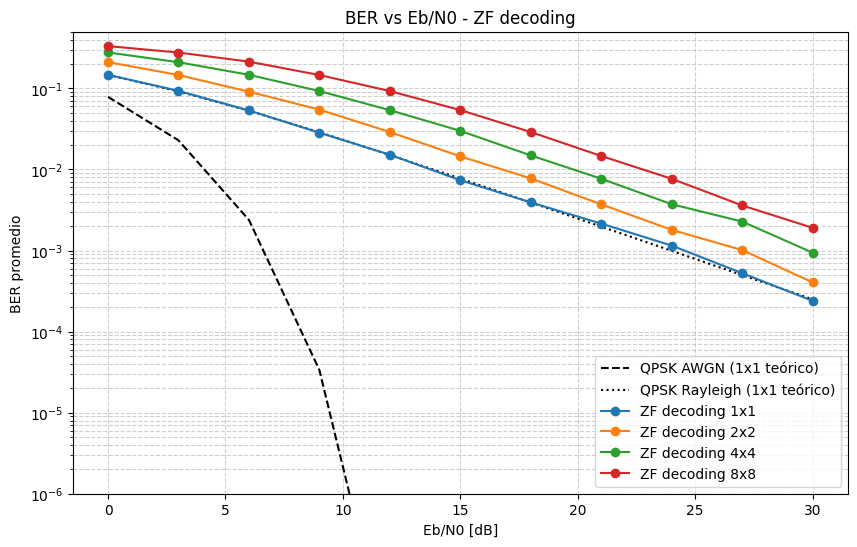
\includegraphics[width=0.95\textwidth]{fig_zf_1x1_2x2_4x4_8x8.png}
    \caption{BER vs $E_b/N_0$ para configuraciones ZF: 1×1, 2×2, 4×4 y 8×8.}
\end{figure}

El desempeño decrece al aumentar el tamaño de la matriz MIMO, debido a que la energía se reparte entre todas las transmisiones simultáneas. Además, la amplificación del ruido inherente al ZF se vuelve más pronunciada en matrices más grandes, afectando negativamente el BER.


% ===========================================
\subsection*{32.c) Simulación ZF para configuraciones 2x1, 4x2 y 8x4}

Se simulan ahora sistemas MIMO sobredimensionados (\(N_r > N_t\)), en los cuales ZF opera en condiciones particularmente favorables.

\begin{figure}[H]
    \centering
    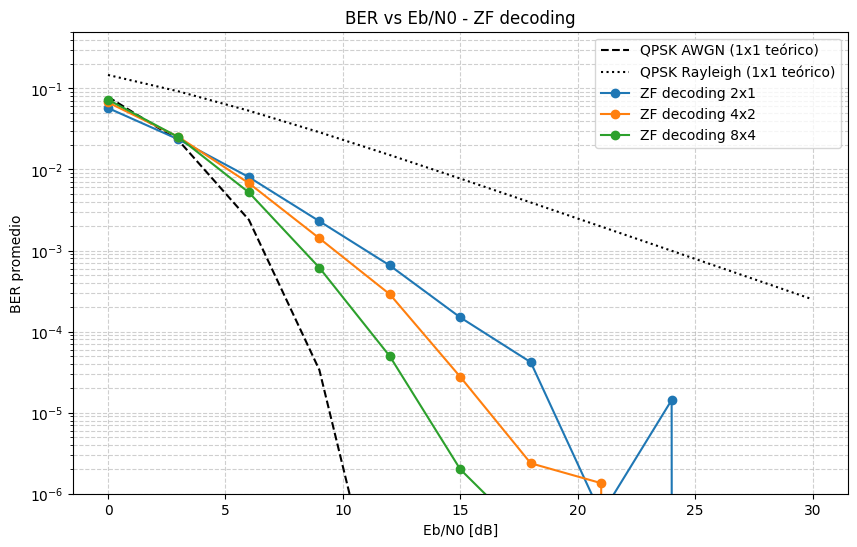
\includegraphics[width=0.95\textwidth]{fig_zf_2x1_4x2_8x4.png}
    \caption{BER vs $E_b/N_0$ para configuraciones ZF: 2×1, 4×2 y 8×4.}
\end{figure}

Las tres configuraciones presentan mejoras notables respecto al caso cuadrado. Tener más antenas receptoras que transmisoras aumenta la dimensionalidad del canal y reduce sustancialmente la amplificación del ruido típica del ZF.


% ================================================================
\section*{Pregunta 33: Decodificación MMSE}

Ahora se repiten exactamente las mismas configuraciones anteriores, pero utilizando \textbf{MMSE}, el cual agrega un término de regularización para mitigar la amplificación de ruido.

% ===========================================
\subsection*{33.a) Simulación MMSE para configuraciones 1x1, 2x1, 4x1 y 8x1}

\begin{figure}[H]
    \centering
    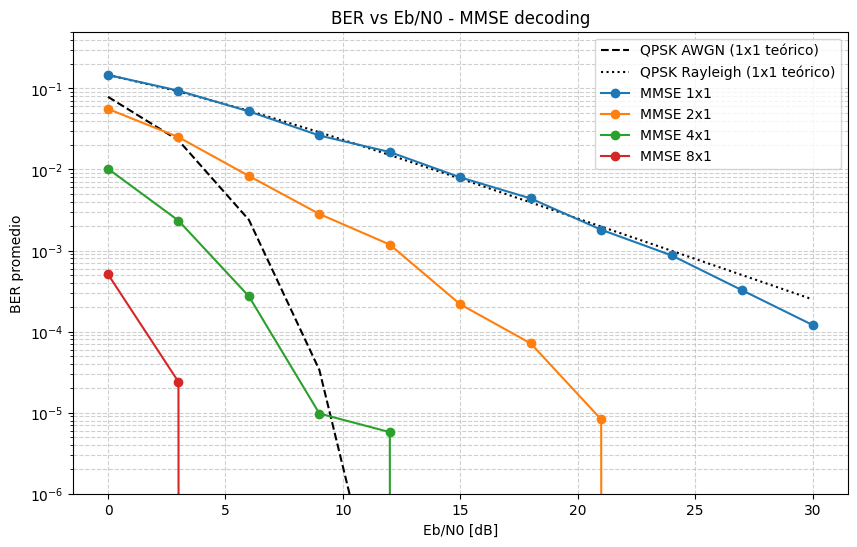
\includegraphics[width=0.95\textwidth]{fig_mmse_1x1_2x1_4x1_8x1.png}
    \caption{BER vs $E_b/N_0$ para configuraciones MMSE: 1×1, 2×1, 4×1 y 8×1.}
\end{figure}

MMSE entrega mejoras considerables en baja SNR respecto a ZF, especialmente visibles en 1×1 y 2×1. El desempeño debería converger al de ZF en alta SNR.


% ===========================================
\subsection*{33.b) Simulación MMSE para configuraciones 1x1, 2x2, 4x4 y 8x8}

\begin{figure}[H]
    \centering
    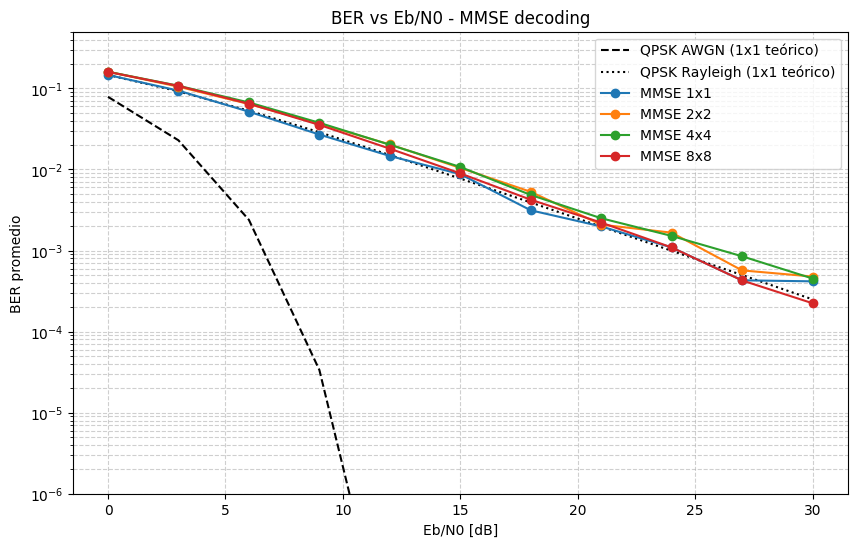
\includegraphics[width=0.95\textwidth]{fig_mmse_1x1_2x2_4x4_8x8.png}
    \caption{BER vs $E_b/N_0$ para configuraciones MMSE: 1×1, 2×2, 4×4 y 8×8.}
\end{figure}

En todos los casos MMSE supera a ZF en la región de baja relación señal-ruido. A medida que crece la matriz MIMO, la diferencia se reduce, dado que la diversidad compensa la amplificación del ruido propia del ZF.


% ===========================================
\subsection*{33.c) Simulación MMSE para configuraciones 2x1, 4x2 y 8x4}

\begin{figure}[H]
    \centering
    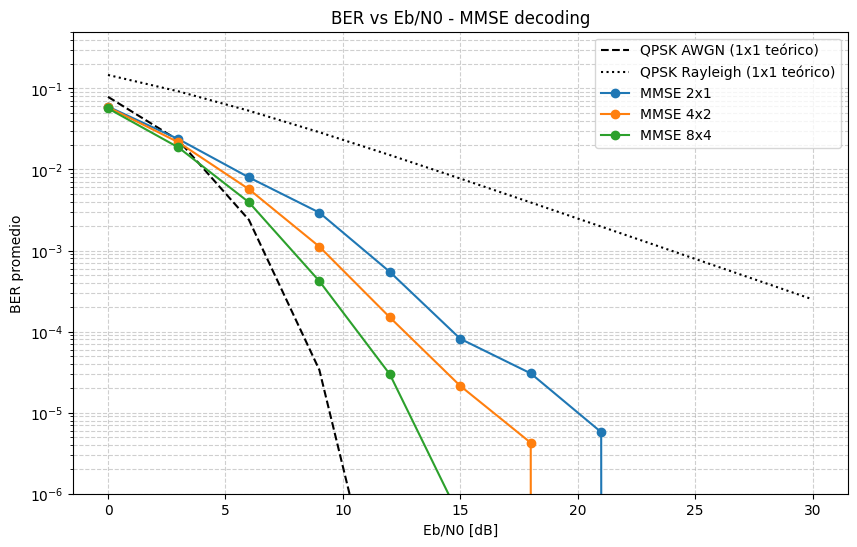
\includegraphics[width=0.95\textwidth]{fig_mmse_2x1_4x2_8x4.png}
    \caption{BER vs $E_b/N_0$ para configuraciones MMSE: 2×1, 4×2 y 8×4.}
\end{figure}

MMSE obtiene la mejor performance relativa en escenarios con más antenas receptoras que transmisoras, dado que puede explotar el exceso de dimensiones para reducir aún más el ruido.


% ======================================================================
\section*{Código utilizado}

\begin{mdframed}
\inputminted{python}{tarea14.py}
\end{mdframed}

\end{document}